\subsection{Lower Bounds}

We're now going to prove that \ref{alg:6-colour} is optimal. Recall that we have the following assumptions:

\begin{itemize}
\item We're working in a synchornous model
\item We have an initial colouring
\end{itemize}

\begin{thm}\label{thm:ring_color_lowerbound} Any deterministic algorithm colouring any\footnote{the only thing that differs between the rings is the initial colouring. We basically claim there exists an initial colouring that produces that runtime.} ring with n nodes with at most three colours needs $\Omega(\log^* n)$ rounds.
\end{thm}

Consider a node $v$. After $t$ rounds it can discover information, i.e. the topology and the IDs, about a $t$-neighbourhood around it.

Assume the vertices can distinguish between clockwise and counterclockwise neighbours, s.t. we can impose some ordering on them (this can only speed up the algorithm, so the assumption is ok for proving lower bounds).

Define

\[W_{s,n} = \{(x_1,x_2,\ldots,x_s) | 1 \leq x_i\leq n, x_i\neq x_j\}\]

Essentially after $t$ rounds, each vertex sees an element from $W_{2t+1,n}$. So any distributed algorithm colouring any right with $\leq 3$ colours calculates a function

\[A:W_{2t+1,n} \longrightarrow \{1,2,3\}\]

in $t$ rounds. We will now show that this function doesn't exist if $t$ is not in $\Omega(\log^*n)$.

Define a graph as follows:

\[G_{s,n} = (W_{s,n},E_{s,n})\]

where there is an edge in between two elements of $W_{s,n}$ in $E_{s,n}$ if they overlap in all but the first and the last position, i.e. edges have the form $\{(x_1,x_2,\ldots,x_s),(x_2,x_3,\ldots,x_{s+1})\}$. So we have edges between neighbourhoods that correspond to neighbouring vertices in some ring.

\begin{figure}[hbt]
\begin{center}
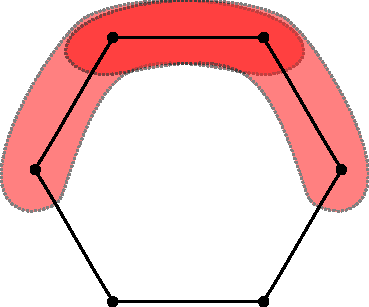
\includegraphics{./images/ring.pdf}
\end{center}
\caption{Overlapping 1-neighbourhoods on a ring}
\end{figure}

\begin{lem} The function $A$ is a valid colouring for the graph $G_{2t+1,n}$.\end{lem}

\begin{pr} Let $\{v,v'\}\in E_{2t+1,n}$ be an edge as above. Assume for the sake of contradiction that $A$ does not produce a valid colouring, i.e. $A(v)=A(v')$. We now construct a ring that is a valid input for the algorithm.

Consider the ring 

\[x_1\rightarrow \ldots \rightarrow x_{t+1} \rightarrow x_{t+2} \rightarrow \ldots \rightarrow x_{2t+1} \rightarrow x_{2t+2} \rightarrow \ldots \rightarrow x_1\] 

%picture ring with vertices x_1... x_t+1 x_t+2 ... x_2t+1,x_2t+2

Since the algorithm produces a valid colouring it colours $x_{t+1}$ and $x_{t+2}$ with different colours. But then the function must be $A(v)\neq A(v')$.
\end{pr}

It follows that $\chi(G_{2t+1,n})\leq 3$. We now show that the chromatic number is actually larger, if $t$ is too small.

\begin{Def} For a graph $\vec G$, the line graph $L(\vec D)$ is  the graph with the same vertex set as $\vec D$ and $(e,e')$ is an edge if e ends where e' starts. 

\begin{figure}[hbt]
\begin{center}
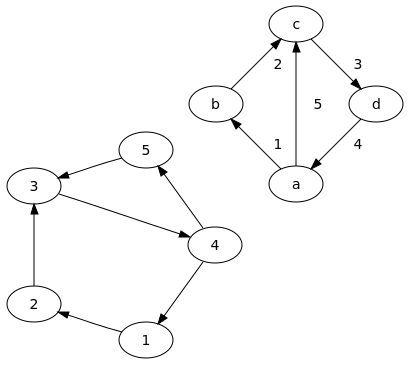
\includegraphics[width=0.8\linewidth]{./images/linegraph_ex}
\end{center}
\caption{A graph and its linegraph}
\end{figure}
\end{Def}

\begin{lem} $\chi(G_{2t+1,n}) \geq \log^{(2t)} n$\end{lem}

\begin{pr} Define a new, directed graph $\vec G_{s,n} = (\vec W_{s,n}, \vec E_{s,n})$ that is build from a subset of the originial graph

\[\vec W_{s,n} = \{(x_1,x_2,\ldots,x_s) | 1\leq x_1\leq \ldots \leq x_s \leq n\}\]
\[\vec E_{s,n} = \{(\underbrace{(x_1,\ldots,x_s)}_{v},\underbrace{(x_2,\ldots,x_{s+1})}_{v'})| v,v'\in \vec W_{s,n} \wedge x_{s+1} > x_s\}\]

Since both the edge and the nodeset of $\vec G$ is a subset of $G$, we immediately have $\chi(\vec G)\leq \chi(G)$. By introducing the new graph we gained the ability to recursively characterize $\vec G_{s,n}$.

\begin{enumerate}
\item $\vec G_{1,n}$ is the complete graph ($i\rightarrow i'$, if $i'>i$). This follows from the definition.
\item $\vec G_{s+1,n} = L(\vec G_{s,n})$

Take $s=3$ as example, see figure \ref{fig:g3_l3}.

\begin{figure}[hbt]
\begin{center}
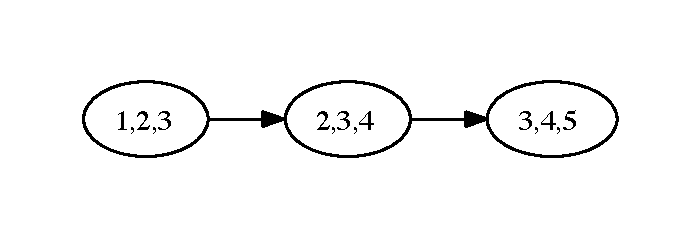
\includegraphics[width=0.58\linewidth]{./images/g3_extr} 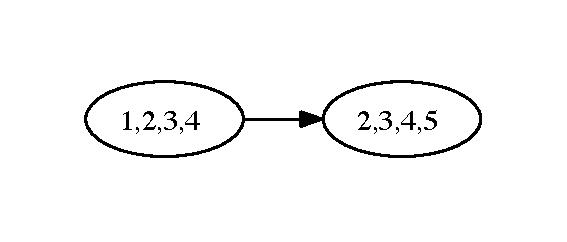
\includegraphics[width=0.4\linewidth]{./images/L(G3)}
\end{center}
\caption{A part of $\vec G_{3,n}$ and the corresponding part of $L(\vec G_{3,n})$}
\label{fig:g3_l3}
\end{figure}

We can identify the edges with elements from $\vec G_4$. And if we don't include an edge in the line graph, we also don't see it in $G_4$.

This also works in the general case: Every time we see an edge in $G_{s,n}$ we map the edge to the union of its endpoints, i.e. a node in $G_{s+1,n}$. If two edges are adjacent s.t. they are a new edge in the line graph, then the union is such that the edge is also in $G_{s+1,n}$
\end{enumerate}
\end{pr}

\begin{lem} $\chi(L(\vec D)) \geq \log \chi(\vec D)$ \end{lem}

\begin{pr} Let $k=\chi(L(\vec D))$ and $\phi$ be a k-colouring. $\phi$ is a colouring of the edges of $\vec D$, since it is a colouring of the line graph.

\begin{center}
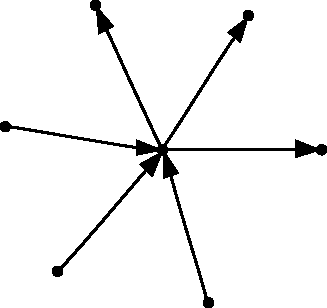
\includegraphics{./images/edge_coloring_line_graph}
\end{center}

For all incoming edges to a, all outgoing edges have a different colour in $\phi$, otherwise it wouldn't be a valid colouring for the line graph.

We construct a colouring $\hat \phi$ of $\vec D$ that uses at most exponentially more colours. 

\[\hat \phi(v) = (b_1,\ldots,x_k)\qquad b_i= \begin{cases} 1 & \exists \text{incoming edge with colour } i\\0 & \text{otherwise}\end{cases}\]

$\hat \phi$ is a valid colouring.

\begin{center}
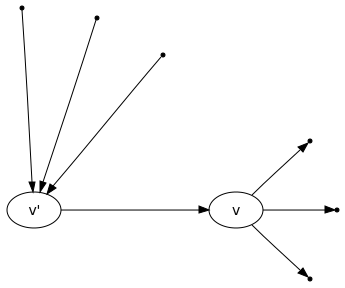
\includegraphics{./images/coloring_from_edges}
\end{center}

Suppose $b_i(v)=1$, then $b_i(v')=0$ otherwise we wouldn't have a valid edge colouring. Since we have $k$ bits available, we can use at most $2^k$ colours in $\hat \phi$.

\end{pr}

\begin{pr}[Theorem \ref{thm:ring_colour_lowerbound}] We need $t=\Omega(\log^* n)$ s.t. $\log^{(2t)} n$ is $\leq 3$.\end{pr}

\paragraph{Remark.}

\begin{itemize} 
\item$G_{s,n}$ doesn't have the nice recursive property. See the example in figure \ref{fig:g_3_counterex}

\begin{figure}[hbt]
\begin{center}
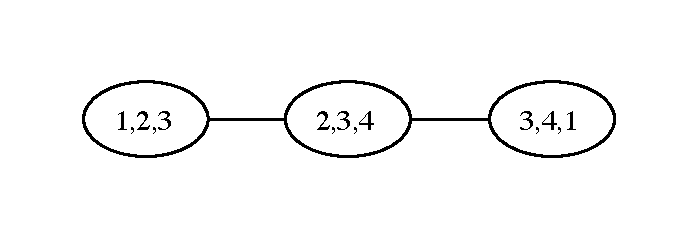
\includegraphics{./images/g_3_counterex}
\end{center}
\caption{The corresponding edge in the line graph $1,2,3,4 \rightarrow 2,3,4,1$ doesn't exist in $G_{4,n}$}
\end{figure}

%1,2,3 -- 2,3,4 -- 3,4,1
%
%a [label ="1,2,3"]
%b [label ="2,3,4"]
%c [label ="3,4,1"]
%
%a -- b -- c
%
%a [label ="1,2,3,4"]
%b [label ="2,3,4,1"]
%a -- b //does not exist
%1,2,3,4 -/- 2,3,4,1
\item The theorem \ref{thm:ring_colour_lowerbound} can be generalised to other graphs too.
\end{itemize}

\section{MIS --- Maximal Independent Set}

\begin{Def} Given an undirected graph $G=(V,E)$ an independent set $U\subseteq V$ is a subset s.t no two vertices in it are connected by an edge:

\[\forall u,v \in U \{u,v\}\not \in E\]

$U$ is \emph{maximal}, if no vertex can be added s.t. this property is preserved. Note the difference to a \emph{maximum} independent set: $U$ is \emph{maximum} if its cardinality is maximal among all independent sets.
\end{Def}

Note that the maximum set anddn a maximal set can be very different 

%picture 
\begin{figure}[hbt]
\begin{center}
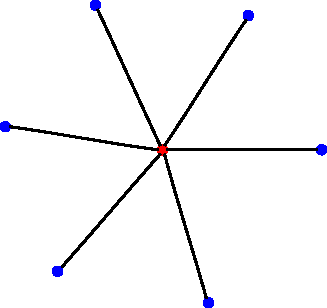
\includegraphics{./images/mis}
\end{center}
\caption{Red node is a maximal independent set, blue are a maximum independent set}
\end{figure}


Finding a maximum independent set is NP-complete, it is even inapproximable by a factor of $\approx \sqrt{n}$ unless P=NP. However maximal independent sets can be computed greedily. We want  to find a distributed algorithm for this problem.

There is a relation between colouring and MIS. Each color class in a coloured graph is an independent set, since there musn't be edges between nodes of the same colour. However it may not be maximal, but we can construct one in a distributed fashion by parallely adding vertices of other colours greedily.

\begin{thm} Given a synchronous distributed algorithm that colours a graph in $R$ rounds with $C$ colours, then we can find a MIS in time $O(R+C)$\qed\end{thm}

\begin{cor} There is a $O(\log^* n)$ algorithm for trees and bounded degree graphs\end{cor}

\subsection{A randomized algorithm}

Here we don't have to assume an initial colouring. Algorithm \ref{alg:fast_mis} runs in phases.

\begin{figure}
\begin{lstlisting}
repeat
	$c$ =  random [0,1] uniformly 
	send $c$ to all neighbour
	
	if $c_v< c_w$ for all $w\in adj(v)$ 
		enter MIS

until $v$ or $w\in adj(v)$ entered
\end{lstlisting}
\caption{Fast-MIS}
\label{alg:fast_mis}
\end{figure}

The algorithm terminates with probability 1, since with probability 1 there is a global smallest random choice, so at least one vertex stops in each round. It also produces a MIS, because as long as a vertex can enter, the algorithm won't stop.

